% Figure from MATH 591 notes, section 1. Compile with the notes preamble.
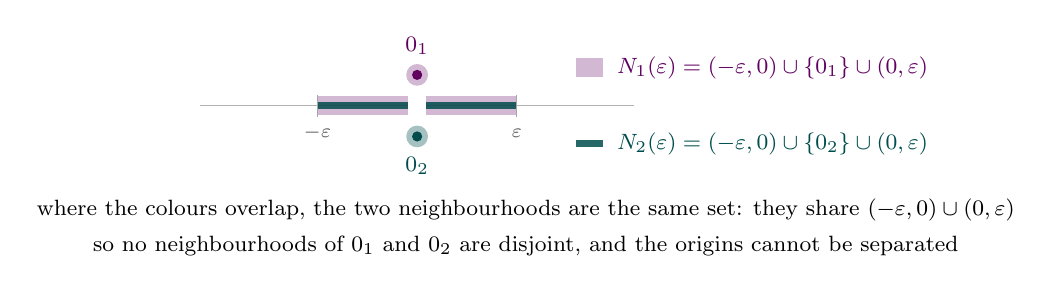
\begin{tikzpicture}[scale=1.15]
% the line, with no ordinary origin
\draw[gray!60] (-2.4,0) -- (-0.1,0); \draw[gray!60] (0.1,0) -- (2.4,0);
% both neighbourhoods painted on the SAME punctured interval: wide purple band, narrow teal band on top
\draw[violet!75!black, line width=7pt, opacity=0.28] (-1.1,0) -- (-0.1,0); \draw[violet!75!black, line width=7pt, opacity=0.28] (0.1,0) -- (1.1,0);
\draw[teal!60!black, line width=2.4pt, opacity=0.85] (-1.1,0) -- (-0.1,0); \draw[teal!60!black, line width=2.4pt, opacity=0.85] (0.1,0) -- (1.1,0);
% the two origins at the gap, each in its own neighbourhood's colour
\fill[violet!75!black, opacity=0.28] (0,0.34) circle (0.12); \fill[violet!75!black] (0,0.34) circle (1.6pt);
\node[violet!75!black,font=\footnotesize,above] at (0,0.46) {$0_1$};
\fill[teal!60!black, opacity=0.35] (0,-0.34) circle (0.12); \fill[teal!60!black] (0,-0.34) circle (1.6pt);
\node[teal!60!black,font=\footnotesize,below] at (0,-0.46) {$0_2$};
% the scale epsilon
\draw[gray!70] (-1.1,-0.12) -- (-1.1,0.12); \draw[gray!70] (1.1,-0.12) -- (1.1,0.12);
\node[font=\scriptsize, text=gray!70!black] at (-1.1,-0.3) {$-\varepsilon$}; \node[font=\scriptsize, text=gray!70!black] at (1.1,-0.3) {$\varepsilon$};
% legend
\draw[violet!75!black, line width=7pt, opacity=0.28] (1.75,0.42) -- (2.05,0.42); \node[violet!75!black,font=\footnotesize,anchor=west] at (2.1,0.42) {$N_1(\varepsilon) = (-\varepsilon,0)\cup\{0_1\}\cup(0,\varepsilon)$};
\draw[teal!60!black, line width=2.4pt, opacity=0.85] (1.75,-0.42) -- (2.05,-0.42); \node[teal!60!black,font=\footnotesize,anchor=west] at (2.1,-0.42) {$N_2(\varepsilon) = (-\varepsilon,0)\cup\{0_2\}\cup(0,\varepsilon)$};
\node[font=\footnotesize] at (1.2,-1.15) {where the colours overlap, the two neighbourhoods are the same set: they share $(-\varepsilon,0)\cup(0,\varepsilon)$};
\node[font=\footnotesize] at (1.2,-1.55) {so no neighbourhoods of $0_1$ and $0_2$ are disjoint, and the origins cannot be separated};
\end{tikzpicture}
